\documentclass[14pt]{extarticle}
\usepackage{fontspec}
\usepackage{polyglossia} % use instead of babel
\usepackage{pgfplots}
\usepackage{float}
\usepackage{amsmath}
\usepackage{amsfonts}
\setdefaultlanguage{hebrew}
\setotherlanguage{english}
\newfontfamily\hebrewfont[Script=Hebrew]{Arial}

% TODO: figure out if better to keep this or not, for word document pdf output similarity
\usepackage[margin=1in]{geometry}

% might be useful to ensure similarity to word document pdf output
% \usepackage{setspace}
% \singlespacing

% Reset equation counter at the start of each section
\usepackage{chngcntr}
\usepackage{etoolbox}
\counterwithin*{equation}{section}
\preto{\section}{\setcounter{equation}{0}}

% Left-aligned equation environment
\newenvironment{lefteqs}{%
    \begin{english}%
    \begin{flushleft}%
    \renewcommand{\arraystretch}{1.3}%
    $\begin{array}{@{}l@{}}%
}{%
    \end{array}$%
    \end{flushleft}%
    \end{english}%
}

\begin{document}

\begin{center}
    {\LARGE \textbf{מעבדה 8}}\\
    {\textbf{מעגלי זרם חילופין}}
\end{center}

\begin{itemize}
    \item מגישים
    \begin{itemize}
        \item אורי כספי - 331496927 
        \item שי רואימי - 318986270
    \end{itemize}
    \item תאריך ביצוע הניסוי: 3 באוגוסט 2026
\end{itemize}
\newpage
\section*{רקע תיאורטי}

\subsection*{ניסוי 1}

מתח חילופין סינוסואידלי הוא מתח שערכו משתנה בזמן לפי פונקציית סינוס
\begin{equation}
    V(t) = V_0 \sin(\omega t + \beta)
\end{equation}
כאשר $V_0$ הוא המשרעת של המתח, $\omega$ הוא התדירות הזוויתית של המתח, $t$ הוא הזמן, ו-$\beta$ הוא המופע ההתחלתי.

רב-מודד אינו מודד את המשרעת אלא את הערך האפקטיבי של המתח והזרם, שהוא פרופורציוני למשרעת.
מאחר שכל המתחים והזרמים קטנים באותו יחס, הקשרים שלהלן תקפים גם עבור הערכים האפקטיביים, וניתן להציב בהם ישירות את קריאות הרב-מודד.

בנגד מתקיים חוק אוהם בכל רגע: $Ri=v$.
מכיוון ש-$R$ הוא קבוע ממשי וחיובי, המתח והזרם נמצאים תמיד באותו המופע (הפרש מופע אפס).
העכבה של נגד ממשית: $Z_R = R [\Omega]$.

בסליל אידיאלי המתח פרופורציוני לקצב שינוי הזרם:
\begin{equation}
    v = L \frac{di}{dt}
\end{equation}
כאשר $L$ היא ההשראות $[H]$.
עבור זרם סינוסואידלי $i=I_m \sin(\omega t)$ מתקיים:
\begin{equation}
    v = L \frac{di}{dt} = L I_m \omega \cos(\omega t) = L I_m \omega \sin(\omega t + \frac{\pi}{2})
\end{equation}
כלומר המתח על הסליל מקדים את הזרם ב$\frac{\pi}{2}$.
גודל ההתנגדות שהסליל מציב לזרם הוא:
\begin{equation}
    X_L = \omega L [\Omega]
\end{equation}
והעכבה המרוכבת היא:
\begin{equation}
    Z_L = j \omega L [\Omega]
\end{equation}
כאשר הגורם המדומה $j$ מבטא את הקדמת המופע ב $\frac{\pi}{2}$.

מכיוון שהרכיבים מחוברים בטור, אותו זרם $i$ זורם דרך שניהם, ולכן נוח לתאר את המתחים כווקטורים ביחס לכיוון הזרם:
$V_R$ נמצא באותו מופע כמו הזרם ואילו $V_L$ מקדים את הזרם ב $\frac{\pi}{2}$ (ניצב לו).

מתח המקור הוא הסכום הווקטורי של השניים. מכיוון ש $V_R$ ו-$V_L$ ניצבים זה לזה, מתקיים:
\begin{equation}
    V = \sqrt{V_R^2 + V_L^2}
\end{equation}
(זה מקרה פרטי כאשר אין קבל במעגל, כלומר $V_C=0$).

העכבה הכוללת במעגל היא:
\begin{equation}
    Z = R + j \omega L [\Omega]
\end{equation}
וגודלה:
\begin{equation}
    |Z| = \sqrt{R^2 + (\omega L)^2} [\Omega]
\end{equation}
הזרם האפקטיבי מחושב לפי חוק אוהם המוכלל:
\begin{equation}
    I = \frac{V}{|Z|}
\end{equation}

הפרש המופע $\theta$ בין מתח המקור לזרם (שהוא גם הפרש המופע בין מתח המקור למתח הנגד) נקבע מהיחס
בין הרכיב הניצב לרכיב שלאורך הזרם:
\begin{equation}
    \tan(\theta) = \frac{V_L}{V_R} = \frac{\omega L}{R}
\end{equation}

בצורה גרפית קל לראות את הקשרים בין המתחים:
\begin{figure}[H]
    \centering
    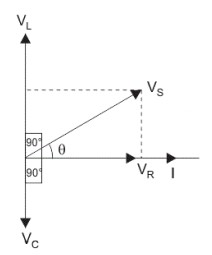
\includegraphics[width=0.3\textwidth]{voltage_graph.jpg}
    \caption{דיאגרמה וקטורית של המתחים במעגל R-L טורי}
\end{figure}

הזזה של זמן $\Delta t$ בין שני אותות בעלי מחזור $T$ שקולה לחלק היחסי $\frac{\Delta t}{T}$ ממחזור שלם ולכן להפרש מופע:
\begin{equation}
    \phi = \frac{\Delta t}{T} \cdot 2\pi = 2 \pi f \Delta t
\end{equation}

\subsection*{ניסוי 2}
הרקע התיאורטי לניסוי זה נשען על הרקע לניסוי 1, ומרחיב אותו לכלול גם קבל.

בקבל אידיאלי הזרם פרופורציוני לקצב שינוי המתח:
\begin{equation}
    i = C \frac{dv}{dt}
\end{equation}
כאשר $C$ הוא הקיבול $[F]$.
עבור מתח סינוסואידלי $v = V_m \sin(\omega t)$ מתקיים:
\begin{equation}
    i = C \frac{dv}{dt} = \omega C V_m \cos(\omega t) = \omega C V_m \sin(\omega t + \frac{\pi}{2})
\end{equation}
כלומר הזרם בקבל מקדים את המתח ב$\frac{\pi}{2}$ (המתח מפגר אחרי הזרם).
גודל ההתנגדות שהקבל מציב לזרם הוא:
\begin{equation}
    X_C = \frac{1}{\omega C} [\Omega]
\end{equation}
והעכבה המרוכבת היא:
\begin{equation}
    Z_C = \frac{1}{j \omega C} = -\frac{j}{\omega C} [\Omega]
\end{equation}
כאשר הסימן המדומה השלילי מבטא את פיגור המתח ב$\frac{\pi}{2}$.

במעגל RLC טורי מחוברים נגד, סליל וקבל בטור, ואותו זרם זורם דרך שלושתם. נתאר את המתחים כווקטורים ביחס לכיוון הזרם באותה שיטה שהוצגה ברקע לניסוי 1, כאשר נוסף כעת המתח על הקבל $V_C$ המפגר אחרי הזרם ב$\frac{\pi}{2}$ (כלפי מטה, מנוגד ל-$V_L$). מאחר ש-$V_L$ ו-$V_C$ מנוגדים בכיוונם, הרכיב הניצב הכולל הוא $V_L - V_C$, ומתח המקור מקיים:
\begin{equation}
    V_S^2 = V_R^2 + (V_L - V_C)^2
\end{equation}
(המקרה של מעגל R-L מתקבל כאשר $V_C = 0$).

בהכללת העכבה מניסוי 1 בתוספת תרומת הקבל, העכבה הכוללת של המעגל היא:
\begin{equation}
    Z = R + j\left(\omega L - \frac{1}{\omega C}\right) [\Omega]
\end{equation}
וגודלה:
\begin{equation}
    |Z| = \sqrt{R^2 + \left(\omega L - \frac{1}{\omega C}\right)^2} [\Omega]
\end{equation}
בדומה לניסוי 1, הפרש המופע בין מתח המקור לזרם נקבע מהיחס בין הרכיב הניצב (כעת $V_L - V_C$) לרכיב שלאורך הזרם:
\begin{equation}
    \tan(\theta) = \frac{V_L - V_C}{V_R} = \frac{\omega L - \frac{1}{\omega C}}{R}
\end{equation}

גודל ההתנגדות של הסליל $X_L = \omega L$ גדל עם התדר, ואילו גודל ההתנגדות של הקבל $X_C = \frac{1}{\omega C}$ קטן עם התדר. בתדר מסוים הם משתווים, החלק המדומה של העכבה מתאפס, והעכבה נעשית אוהמית טהורה ומינימלית ($Z = R_T$). מצב זה נקרא תהודה. תנאי התהודה $\omega L = \frac{1}{\omega C}$ נותן את תדירות התהודה:
\begin{equation}
    \omega_0 = \frac{1}{\sqrt{LC}} \left[\frac{rad}{s}\right], \qquad f_0 = \frac{\omega_0}{2\pi} = \frac{1}{2\pi\sqrt{LC}} [Hz]
\end{equation}
בתהודה העכבה מינימלית ולכן הזרם מקסימלי, והפרש המופע בין הזרם למתח המקור מתאפס. כאן $R_T$ היא ההתנגדות האקטיבית הכוללת במעגל, הכוללת את הנגד $R$ ואת ההתנגדות האקטיבית של הסליל $R_{in}$:
\begin{equation}
    R_T = R + R_{in} [\Omega]
\end{equation}

רוחב הסרט $\Delta\omega$ הוא תחום התדירויות שבו גודל הזרם אינו יורד מתחת ל$\frac{1}{\sqrt{2}}$ מערכו המרבי:
\begin{equation}
    \Delta\omega = \frac{R_T}{L} \left[\frac{rad}{s}\right]
\end{equation}

טיב המעגל (גורם האיכות) $Q$ מודד את חדות עקומת התהודה, ומוגדר כיחס בין גודל ההתנגדות של הסליל בתהודה, $\omega_0 L$, להתנגדות האקטיבית הכוללת $R_T$:
\begin{equation}
    Q = \frac{\omega_0}{\Delta\omega} = \frac{\omega_0 L}{R_T} = \frac{1}{\omega_0 R_T C} = \frac{1}{R_T}\sqrt{\frac{L}{C}}
\end{equation}

המתחים על הרכיבים כתלות בתדר נקראים עקומות היענות (אופייני תהודה). הערכים המקסימליים של המתח על הקבל ועל הסליל מתקבלים בתדרים השונים מעט מתדר התהודה:
\begin{equation}
    \omega_C = \omega_0 \sqrt{1 - \frac{1}{2Q^2}} < \omega_0
\end{equation}
\begin{equation}
    \omega_L = \frac{\omega_0}{\sqrt{1 - \frac{1}{2Q^2}}} > \omega_0
\end{equation}
ככל ש-$Q$ גדול יותר, $\omega_C$ ו-$\omega_L$ מתקרבים ל-$\omega_0$ ועקומות ההיענות חדות יותר.

\section*{ניסוי 1 - מעגל RL טורי}

\subsection*{מטרת הניסוי}
\begin{itemize}
    \item לחקור התנהגות של מעגל R-L טורי מחובר למקור מתח חילופין
    \item מדידת הפרש המופע בין מתח המקור לבין הזרם במעגל
    \item בדיקת התלות בין המתחים על רכיבים במעגל לבין תדר מתח המקור
\end{itemize}

\subsection*{מהלך הניסוי}

הרכבנו מעגל R-L טורי כמתואר באיור 8:
\begin{figure}[H]
    \centering
    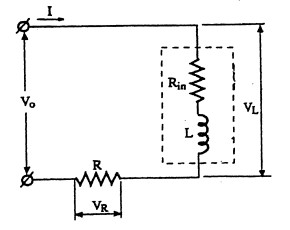
\includegraphics[width=0.3\textwidth]{book_figure_8.jpg}
    \caption{מעגל R-L טורי}
\end{figure}


נגד בעל התנגדות $R = 470\,\Omega$ וסליל בעל השראות $L = 8.2\,\text{mH}$.

הסליל אינו אידיאלי, ולכן בתחילת הניסוי מדדנו בעזרת רב-מודד את ההתנגדות האקטיבית שלו.
 
לאחר מכן חיברנו את המעגל, כאשר המחולל מחובר לערוץ 1 באוסילוסקופ, והנגד מחובר לערוץ 2.
 
כיוונו את המחולל למתח סינוסודיאלי בתדר של $10\, \text{kHz}$.

באוסילוסקופ מיקמונו Cursor A במקום בו מתח המקור מתאפס ואת Cursor B בנקודה בה הנגד מתאפס, וככה מדדנו את הפרש הזמנים בין האותות $\Delta t$.
בעזרת $Delta t$ חישבנו את הפרש המופע בין האותות.

לאחר מכן ניתקנו את החיבורים לאוסילוסקופ, וחיברנו רב מודד לכל אחד מהרכיבים במעגל (מחולל אותות, נגד וסליל).
לכל אחד מהתדרים $1 \text{kHz}$, $2\text{kHz}$, $4\text{kHz}$, $10\text{kHz}$, מדדנו את ערכי המתח על כל אחד מהרכיבים ואת הזרם במעגל.

\subsection*{תוצאות וניתוח}
\subsection*{דיון ומסקנות}


\section*{ניסוי 2 - מעגל RLC (תהודה)}
\subsection*{מטרת הניסוי}
\begin{itemize}
    \item לחקור את תופעת התהודה במעגל RLC טורי המחובר למקור מתח חילופין.
    \item למצוא את תדר התהודה של המעגל בעזרת אוסילוסקופ, ולהשוותו לערך התיאורטי המחושב מערכי הרכיבים.
    \item למדוד את עקומות ההיענות של המתחים על הנגד, הסליל והקבל כתלות בתדר
    \item לחשב את טיב המעגל $Q$ ואת התדרים שבהם המתח על הסליל ועל הקבל מגיע למקסימום
\end{itemize}

\subsection*{מהלך הניסוי}

הרכבנו מעגל RLC טורי כמתואר באיור 9 במדריך הניסוי:

\begin{figure}[H]
    \centering
    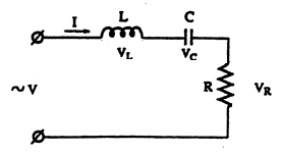
\includegraphics[width=0.3\textwidth]{book_figure_9.jpg}
    \caption{מעגל RLC טורי}
\end{figure}

נגד בעל התנגדות $R = 100\,\Omega$, סליל בעל השראות $L = 8.2\,\text{mH}$ וקבל בעל קיבול $C = 0.047\,\mu\text{F}$

חיברנו את הרכיבים בטור למחולל אותות, שהגדרנו לגל סינוס. את המחולל חיברנו לערוץ 1 של האוסילוסקופ ואת הנגד לערוץ 2 (חיבור במקביל).

לאחר מכן שנינו את תדר המחולל עד שקיבלנו תדר תהודה. את תדר התהודה זיהינו לפי כך שהמתח על הנגד (המייצג את הזרם במעגל) הגיע למשרעת מקסימלית ונמצא באותו מופע כמתח המקור, כלומר הפרש המופע ביניהם התאפס.

לאחר מכן נתקנו את החיבורים לאוסילוסקופ וחיברנו רב מודד לכל אחד מהרכיבים במעגל, ועבור טווח תדרים מדדנו את המתחים של כל הרכיבים.

טווח התדרים התחיל מתדר התהודה, כאשר עלינו וגם ירדנו בקפיצות של $100 \text{Hz}$ סביב תדר התהודה, וכאשר התרחקנו ממנו מספיק, בקפיצות של $500 \text{Hz}$.

יש לציין שבתהליך שינוי התדר שנינו את אמפליטודת המחולל כך שמתח היציאה במחולל ישאר קבוע.

\subsection*{תוצאות וניתוח}
\subsection*{דיון ומסקנות}


\end{document}